\section{Planning}
This part describes all the planning carried out during the development of this project, detailing the different meetings and iterations performed. In figure  \ref{fig:gantt} the following \textbf{\textit{Gantt}} diagram can be seen where the different phases of the project are indicated.
\begin{figure}[H]
    \centering
    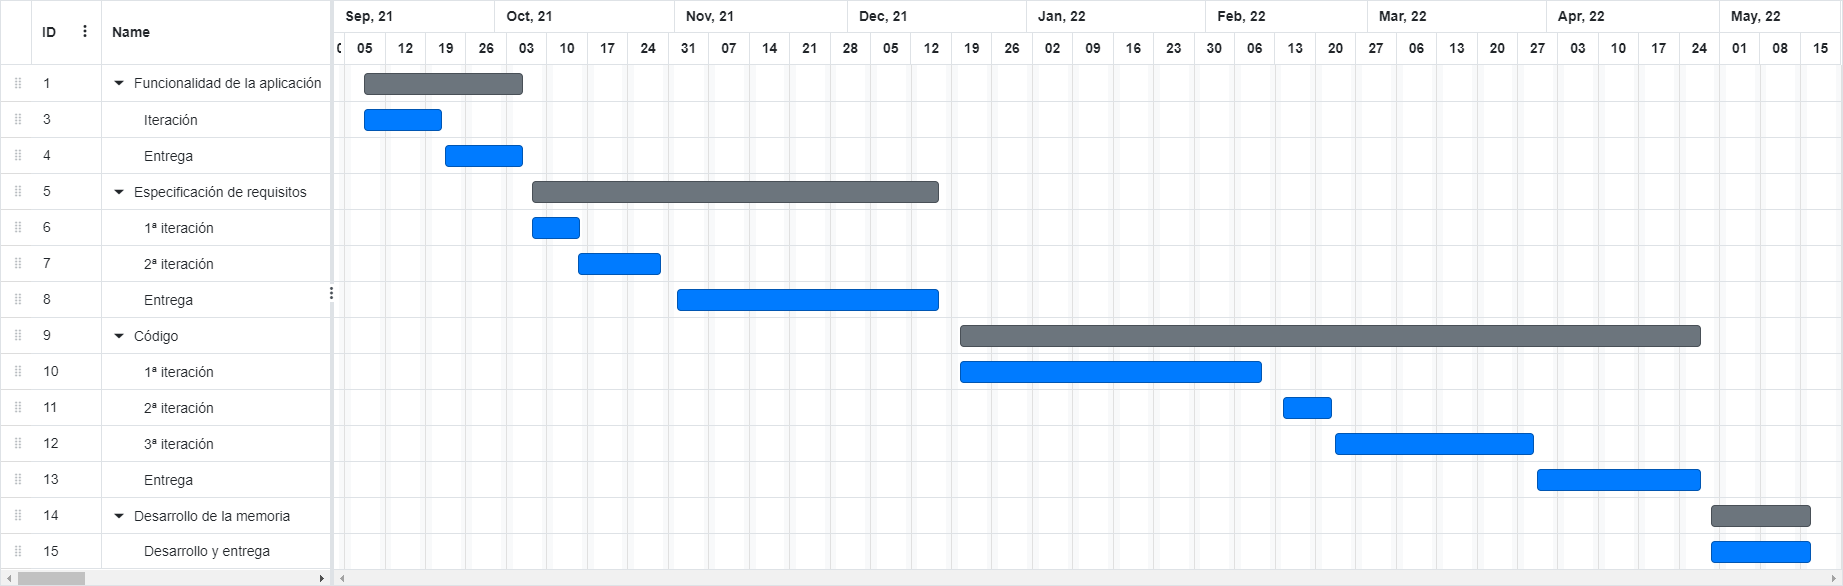
\includegraphics[width=\textwidth]{Images/gantt.png}
    \caption{Gantt chart of project planning}
    \label{fig:gantt}
\end{figure}

During the first phase, the main functionalities of the application were established. Once this phase was completed, the requirements were specified as well as the actors and modules that make up the application. Two iterations were carried out in order to establish the final requirements.

Subsequently, three code iterations were established, in each of which the different modules previously established (login, diet, current diet) were developed. After the code iterations, different white box tests were performed on the different use cases. In the last phase, the memory that complements the code was developed.

In order to carry out the different phases mentioned above, the team held meetings every Saturday, in order to establish the functionality to be developed during the week. At the same time, the meetings helped to know what the team members had done during the previous week, as well as to try to solve together the problems that arose.